\documentclass[convert]{standalone}

\usepackage{tikz}
\usepackage{standalone}
\usepackage{tikz-feynman}

\begin{document}

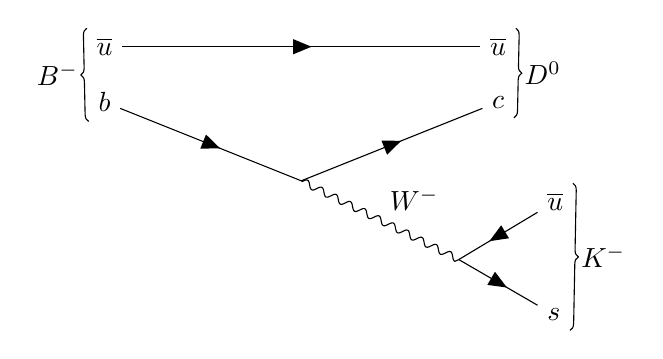
\begin{tikzpicture}
    \begin{feynman}
        \vertex (uBarIn) {\(\overline{u}\)};
        \vertex[right=5cm of uBarIn] (uBarOut) {\(\overline{u}\)};
        \vertex[below=2em of uBarIn] (b) {\(b\)};
        \vertex[right=5cm of b] (c) {\(c\)};
        \vertex[below right=1cm and 2.5cm of b] (v1);
        \vertex[below right=1cm and 2cm of v1] (v2);
        \vertex[above right=0.5cm and 1cm of v2] (uBar) {\(\overline{u}\)};
        \vertex[below right=0.5cm and 1cm of v2] (s) {\(s\)};
        \diagram* { {[edges=fermion]
                (uBarIn) -- (uBarOut),
                (b) -- (v1) -- (c), (uBar) -- (v2) -- (s)},
        (v1) -- [boson, edge label=\(W^-\)] (v2)
        };
        \draw [decoration={brace}, decorate] (b.south west) -- (uBarIn.north west) node [pos=0.5, left] {\(B^-\)};
        \draw [decoration={brace}, decorate] (uBarOut.north east) --  (c.south east) node [pos=0.5, right] {\(D^0\)};
        \draw [decoration={brace}, decorate] (uBar.north east) --  (s.south east) node [pos=0.5, right] {\(K^-\)};
    \end{feynman}
\end{tikzpicture}

\end{document}
